\chapter{Introduction}
\label{chap:intro}
Probabilistic programs are “usual” programs (written in languages like C, Java, LISP or ML) with two added constructs: (1) the ability to draw values at random from distributions, and (2) the ability to condition values of variables in a program via observe statements (which allow data from real world observations to be incorporated into a probabilistic program). A variety of probabilistic programming languages and systems have been proposed including BUGS ~\cite{bugs}, Church [~\cite{church}, FACTORIE ~\cite{factorie}, Infer.NET ~\cite{infernet}, Dimple ~\cite{dimple}, etc. However, unlike “usual” programs which are written for the purpose of being executed, the purpose of a probabilistic program is to implicitly specify a probability distribution. Probabilistic programs can be used to represent probabilistic graphical models ~\cite{pgm}, which use graphs to denote conditional dependences between random variables. Probabilistic graphical models are widely used in statistics and machine learning, with diverse application areas including information extraction, speech recognition, computer vision, coding theory, biology and reliability analysis.

Probabilistic inference is the problem of computing an explicit representation of the probability distribution implicitly specified by a probabilistic program. If the probability distribution is over a large number of variables, an explicit representation of the joint probability distribution may be both difficult to obtain efficiently, and unnecessary in the context of specific application contexts. For example, we may want to compute the expected value of some function f with respect to the distribution (which may be more efficient to calculate without representing the entire joint distribution). Alternatively, we may want to calculate the most likely value of the variables, which is the mode of the distribution. Or we may want to simply draw a set of samples from the distribution, to test some other system which expects inputs to follow the modeled distribution.

The area of probabilistic programming is becoming more and more popular in recent years with more and more publications in top conferences such as NIPS and POPL, attracting researchers from universities such as MIT and Stanford and industry research institutions such as Microsoft Research. However, to our best knowledge, this area has not even been studied in China. 
The goal of the probabilistic programming is to make machine learning model code shorter, to reduce development time, to facilitate the construction of richer models, to require lower levels of expertise in building machine learning applications, and to support the construction of integrated models. In Probabilistic programming, modeling and inference have been disentangled. An example of the probabilistic programs for LDA is showed in Figure ~\ref{fig:lda}.

\begin{figure}
    \centering
    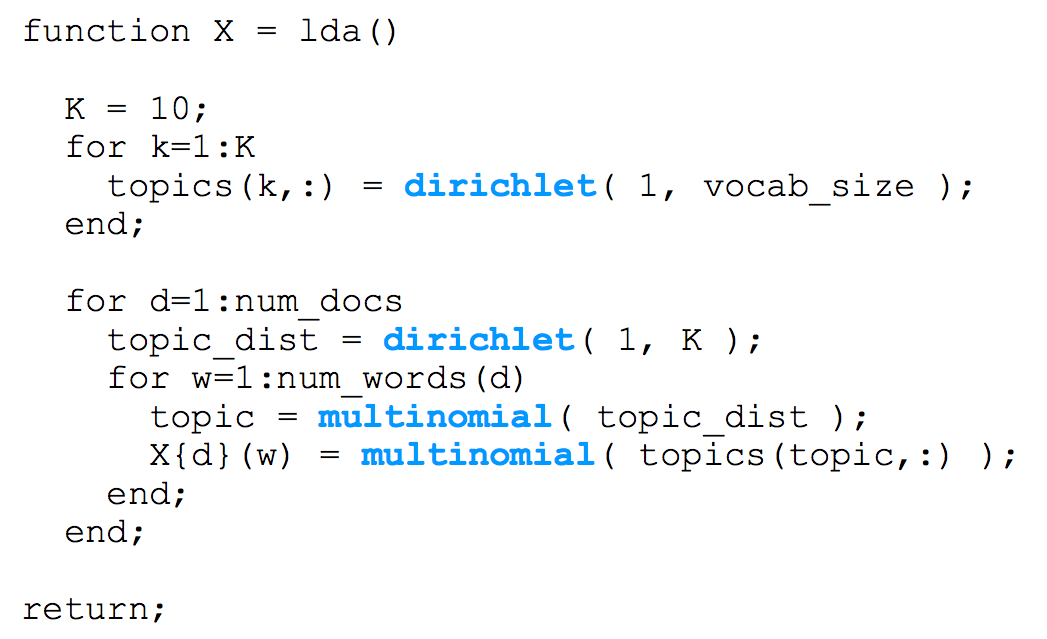
\includegraphics[width=0.9\textwidth]{figures/lda_eg.png}
    \caption{Probabilistic program example: LDA.}
    \label{fig:lda}
\end{figure}

Currently there are many probabilistic programming languages and systems. We have evaluated the existing probabilistic programming systems including BUGS ~\cite{bugs}, Church ~\cite{church}, FACTORIE ~\cite{factorie}, Infer.NET ~\cite{infernet}, Dimple ~\cite{dimple}, etc. More specifically, BUGS is a language for specifying finite graphical models and accompanying software for performing Bayesian inference Using Gibbs Sampling. Church is a universal probabilistic programming language, extending Scheme with probabilistic semantics, and is well suited for describing infinite-dimensional stochastic processes and other recursively-defined generative processes. Factorial is a Scala library for creating relational factor graphs, estimating parameters and performing inference. Infer.NET is a software library developed by Microsoft for expressing graphical models and implementing Bayesian inference using a variety of algorithms within the .NET platform. Dimple is a software tool that performs inference and learning on probabilistic graphical models via belief propagation algorithms or sampling based algorithms. In summary, all these probabilistic programming languages are extended from a domain language and each of them inherits the same syntax and the data types of the domain language. 

Although currently there are many probabilistic programming languages and systems, as stated above, the problem is that this is not easy for those cross-platform developments where they have to get accustomed to the different kinds of probabilistic programming languages or libraries. Henceforth, what we proposed is the Portable Probabilistic Programming Framework that can be embedded in every programming language people commonly used.

We designed the syntax for the portable probabilistic programming language which targets Bayesian networks and conditional query. The design of the language is based on BUGS and is more specific and efficient for describing the probabilistic models. The description of the models using the portable probabilistic programming language is separated from the code of the host language as well of the conditional query, which can enhance the reusability of the probabilistic models. The parser is implemented and the inference engine is generated automatically based on the conditional query. The inference algorithm is based on the MCMC sampling, such as Gibbs Sampling or Metropolis-Hastings Algorithm, which is efficient and lightweight to implement. Additionally, the APIs for other languages is attached leveraging some existing development tool such as SWIG (Simplified Wrapper and Interface Generator). 

Our main contribution lies in the design of the portable probabilistic programming language to make it portable, the implementation of the probabilistic library and the lightweight implementation of the inference engine. 

In Chapter ~\ref{chap:approach}, we will elaborate on the approach of the design and implementation of the portable probabilistic programming framework. More specifically, the syntax of the language is illustrated in section ~\ref{sec:syntax} and the implementation of the probabilistic library is showed in section ~\ref{sec:distr}. The algorithms of probabilistic inference and the implementation of the inference engine are elaborated in section ~\ref{sec:infer}. And the implementation of the APIs for other common programming languages is illustrated in section ~\ref{sec:api}. In Chapter ~\ref{chap:conclusion}, we will conclude our work and the future work that can be done based our framework. In Chapter ~\ref{chap:related}, the related work will be introduced.
